% Options for packages loaded elsewhere
\PassOptionsToPackage{unicode}{hyperref}
\PassOptionsToPackage{hyphens}{url}
%
\documentclass[
]{book}
\usepackage{amsmath,amssymb}
\usepackage{lmodern}
\usepackage{iftex}
\ifPDFTeX
  \usepackage[T1]{fontenc}
  \usepackage[utf8]{inputenc}
  \usepackage{textcomp} % provide euro and other symbols
\else % if luatex or xetex
  \usepackage{unicode-math}
  \defaultfontfeatures{Scale=MatchLowercase}
  \defaultfontfeatures[\rmfamily]{Ligatures=TeX,Scale=1}
\fi
% Use upquote if available, for straight quotes in verbatim environments
\IfFileExists{upquote.sty}{\usepackage{upquote}}{}
\IfFileExists{microtype.sty}{% use microtype if available
  \usepackage[]{microtype}
  \UseMicrotypeSet[protrusion]{basicmath} % disable protrusion for tt fonts
}{}
\makeatletter
\@ifundefined{KOMAClassName}{% if non-KOMA class
  \IfFileExists{parskip.sty}{%
    \usepackage{parskip}
  }{% else
    \setlength{\parindent}{0pt}
    \setlength{\parskip}{6pt plus 2pt minus 1pt}}
}{% if KOMA class
  \KOMAoptions{parskip=half}}
\makeatother
\usepackage{xcolor}
\IfFileExists{xurl.sty}{\usepackage{xurl}}{} % add URL line breaks if available
\IfFileExists{bookmark.sty}{\usepackage{bookmark}}{\usepackage{hyperref}}
\hypersetup{
  pdftitle={Méthodes numériques},
  pdfauthor={Bruno Duchesne},
  hidelinks,
  pdfcreator={LaTeX via pandoc}}
\urlstyle{same} % disable monospaced font for URLs
\usepackage{longtable,booktabs,array}
\usepackage{calc} % for calculating minipage widths
% Correct order of tables after \paragraph or \subparagraph
\usepackage{etoolbox}
\makeatletter
\patchcmd\longtable{\par}{\if@noskipsec\mbox{}\fi\par}{}{}
\makeatother
% Allow footnotes in longtable head/foot
\IfFileExists{footnotehyper.sty}{\usepackage{footnotehyper}}{\usepackage{footnote}}
\makesavenoteenv{longtable}
\usepackage{graphicx}
\makeatletter
\def\maxwidth{\ifdim\Gin@nat@width>\linewidth\linewidth\else\Gin@nat@width\fi}
\def\maxheight{\ifdim\Gin@nat@height>\textheight\textheight\else\Gin@nat@height\fi}
\makeatother
% Scale images if necessary, so that they will not overflow the page
% margins by default, and it is still possible to overwrite the defaults
% using explicit options in \includegraphics[width, height, ...]{}
\setkeys{Gin}{width=\maxwidth,height=\maxheight,keepaspectratio}
% Set default figure placement to htbp
\makeatletter
\def\fps@figure{htbp}
\makeatother
\setlength{\emergencystretch}{3em} % prevent overfull lines
\providecommand{\tightlist}{%
  \setlength{\itemsep}{0pt}\setlength{\parskip}{0pt}}
\setcounter{secnumdepth}{5}
\usepackage{booktabs}
\ifLuaTeX
  \usepackage{selnolig}  % disable illegal ligatures
\fi
\usepackage[]{natbib}
\bibliographystyle{plainnat}

\title{Méthodes numériques}
\author{Bruno Duchesne}
\date{2022-04-07}

\usepackage{amsthm}
\newtheorem{theorem}{Théorème}[chapter]
\newtheorem{lemma}{Lemme}[chapter]
\newtheorem{corollary}{Corollaire}[chapter]
\newtheorem{proposition}{Proposition}[chapter]
\newtheorem{conjecture}{Conjecture}[chapter]
\theoremstyle{definition}
\newtheorem{definition}{Définition}[chapter]
\theoremstyle{definition}
\newtheorem{example}{Exemple}[chapter]
\theoremstyle{definition}
\newtheorem{exercise}{Exercice}[chapter]
\theoremstyle{definition}
\newtheorem{hypothesis}{Hypothèse}[chapter]
\theoremstyle{remark}
\newtheorem*{remark}{Remarque}
\newtheorem*{solution}{Solution}
\begin{document}
\maketitle

{
\setcounter{tocdepth}{1}
\tableofcontents
}
\hypertarget{introduction}{%
\chapter*{Introduction}\label{introduction}}
\addcontentsline{toc}{chapter}{Introduction}

Lorem ipsum dolor sit amet, consectetur adipiscing elit, sed do eiusmod tempor incididunt ut labore et dolore magna aliqua. Amet luctus venenatis lectus magna fringilla. Purus in mollis nunc sed id semper risus. Enim facilisis gravida neque convallis a cras semper auctor neque. Arcu non odio euismod lacinia at quis risus. Pulvinar sapien et ligula ullamcorper malesuada proin. Tellus elementum sagittis vitae et leo duis ut diam quam. Tellus cras adipiscing enim eu turpis egestas pretium aenean. Id leo in vitae turpis massa sed elementum. Vulputate enim nulla aliquet porttitor lacus luctus. Faucibus pulvinar elementum integer enim neque volutpat ac. Adipiscing vitae proin sagittis nisl rhoncus mattis rhoncus urna. Et tortor consequat id porta nibh venenatis. Pretium viverra suspendisse potenti nullam ac tortor vitae purus. Lacus viverra vitae congue eu consequat ac felis donec et. Enim facilisis gravida neque convallis a cras semper. Eu scelerisque felis imperdiet proin fermentum. Amet mattis vulputate enim nulla aliquet porttitor lacus. Risus commodo viverra maecenas accumsan lacus vel. Aliquet nec ullamcorper sit amet risus nullam eget felis eget.

Amet porttitor eget dolor morbi non arcu risus quis. Sed lectus vestibulum mattis ullamcorper velit. Feugiat scelerisque varius morbi enim nunc faucibus a pellentesque sit. Habitasse platea dictumst quisque sagittis. Elit ut aliquam purus sit amet. Ut consequat semper viverra nam libero justo laoreet sit amet. Et malesuada fames ac turpis egestas integer eget aliquet. Varius sit amet mattis vulputate. Pretium nibh ipsum consequat nisl vel pretium lectus quam id. Quam elementum pulvinar etiam non. Purus in massa tempor nec feugiat nisl pretium fusce id. Ornare suspendisse sed nisi lacus sed viverra tellus in hac. Dictum fusce ut placerat orci nulla pellentesque. Nisi lacus sed viverra tellus in hac habitasse platea. Elit sed vulputate mi sit. Dignissim enim sit amet venenatis urna cursus eget nunc scelerisque. Mattis molestie a iaculis at erat pellentesque.

At ultrices mi tempus imperdiet nulla malesuada pellentesque elit. Justo laoreet sit amet cursus sit amet dictum sit. Etiam dignissim diam quis enim lobortis. Dui accumsan sit amet nulla facilisi. Nisl vel pretium lectus quam id leo. Nibh tortor id aliquet lectus proin nibh nisl. Et odio pellentesque diam volutpat commodo sed egestas egestas fringilla. Tortor at risus viverra adipiscing. Odio aenean sed adipiscing diam donec adipiscing tristique risus nec. Placerat duis ultricies lacus sed turpis tincidunt id. Malesuada fames ac turpis egestas integer eget. Nunc lobortis mattis aliquam faucibus purus in. Pretium fusce id velit ut tortor pretium. Magnis dis parturient montes nascetur ridiculus. Convallis tellus id interdum velit laoreet id donec ultrices.

In pellentesque massa placerat duis ultricies lacus sed turpis. Duis convallis convallis tellus id. Ut aliquam purus sit amet luctus venenatis lectus. At erat pellentesque adipiscing commodo elit. Nam aliquam sem et tortor consequat. Ultrices eros in cursus turpis massa tincidunt dui. Bibendum at varius vel pharetra vel turpis. Viverra ipsum nunc aliquet bibendum enim. Dictum varius duis at consectetur lorem donec massa sapien. Sagittis id consectetur purus ut faucibus. Tristique senectus et netus et malesuada fames ac. Sed nisi lacus sed viverra tellus in. Tellus at urna condimentum mattis pellentesque id nibh tortor. Pulvinar etiam non quam lacus suspendisse faucibus. Phasellus vestibulum lorem sed risus ultricies tristique nulla. Faucibus in ornare quam viverra orci sagittis eu volutpat odio. Sit amet dictum sit amet justo donec enim diam vulputate.

Felis eget nunc lobortis mattis aliquam faucibus purus. Nunc scelerisque viverra mauris in aliquam sem fringilla ut morbi. Egestas sed sed risus pretium quam vulputate dignissim. Mattis rhoncus urna neque viverra justo nec. Sed egestas egestas fringilla phasellus faucibus scelerisque. Dui nunc mattis enim ut. Vestibulum rhoncus est pellentesque elit. Euismod in pellentesque massa placerat duis ultricies. Est lorem ipsum dolor sit amet consectetur adipiscing. Non diam phasellus vestibulum lorem sed risus ultricies tristique nulla. Suspendisse faucibus interdum posuere lorem.

Consequat nisl vel pretium lectus quam id leo. Tortor vitae purus faucibus ornare. Id ornare arcu odio ut sem nulla pharetra diam. Neque sodales ut etiam sit amet nisl purus. Nulla posuere sollicitudin aliquam ultrices. Et tortor at risus viverra. Nulla pharetra diam sit amet nisl. Faucibus vitae aliquet nec ullamcorper sit amet risus. Et magnis dis parturient montes nascetur ridiculus mus mauris vitae. Placerat duis ultricies lacus sed. Duis tristique sollicitudin nibh sit amet commodo nulla. Morbi non arcu risus quis varius quam quisque id. Rhoncus est pellentesque elit ullamcorper dignissim. At auctor urna nunc id cursus metus aliquam eleifend mi. Pretium vulputate sapien nec sagittis aliquam malesuada bibendum arcu vitae. Faucibus scelerisque eleifend donec pretium. Lectus nulla at volutpat diam ut venenatis tellus in metus.

Ut tristique et egestas quis ipsum suspendisse ultrices gravida. Sit amet consectetur adipiscing elit. Diam vel quam elementum pulvinar etiam non quam. Nunc mi ipsum faucibus vitae aliquet nec ullamcorper sit amet. Neque vitae tempus quam pellentesque. Morbi tincidunt augue interdum velit. Nibh tellus molestie nunc non blandit massa enim nec. In fermentum posuere urna nec. Sollicitudin tempor id eu nisl nunc mi ipsum. Mattis ullamcorper velit sed ullamcorper morbi tincidunt. Accumsan lacus vel facilisis volutpat. Sit amet facilisis magna etiam. At elementum eu facilisis sed odio morbi quis commodo.

Sagittis purus sit amet volutpat. A erat nam at lectus urna duis. Consectetur lorem donec massa sapien faucibus et molestie ac feugiat. Nec feugiat nisl pretium fusce id. Mi in nulla posuere sollicitudin aliquam ultrices. Augue eget arcu dictum varius. Pellentesque massa placerat duis ultricies lacus sed turpis tincidunt. Feugiat in ante metus dictum. Condimentum lacinia quis vel eros donec ac odio tempor orci. Ut eu sem integer vitae justo eget magna fermentum iaculis. Eget duis at tellus at urna condimentum mattis pellentesque. Tellus molestie nunc non blandit massa enim. Ac turpis egestas sed tempus. Bibendum ut tristique et egestas quis ipsum suspendisse ultrices. Aliquet enim tortor at auctor urna nunc. Tortor at risus viverra adipiscing at in tellus. Egestas pretium aenean pharetra magna ac. Suspendisse faucibus interdum posuere lorem ipsum dolor sit amet consectetur. Ut pharetra sit amet aliquam id diam maecenas ultricies. Neque aliquam vestibulum morbi blandit cursus risus at ultrices mi.

Augue interdum velit euismod in pellentesque massa. Augue interdum velit euismod in pellentesque massa placerat duis ultricies. Blandit volutpat maecenas volutpat blandit aliquam etiam. Scelerisque in dictum non consectetur a erat. Cras pulvinar mattis nunc sed blandit libero volutpat sed cras. Fusce id velit ut tortor. Curabitur gravida arcu ac tortor dignissim convallis aenean et tortor. Porttitor massa id neque aliquam vestibulum. Vulputate ut pharetra sit amet aliquam. Tempor orci eu lobortis elementum nibh tellus molestie nunc non.

Ut morbi tincidunt augue interdum velit euismod. Augue interdum velit euismod in pellentesque massa placerat duis. Cras semper auctor neque vitae tempus quam pellentesque. Tellus id interdum velit laoreet id donec. Mattis rhoncus urna neque viverra. Nascetur ridiculus mus mauris vitae. Elit ut aliquam purus sit amet luctus. Ridiculus mus mauris vitae ultricies leo integer malesuada. In mollis nunc sed id semper risus in hendrerit gravida. Pulvinar etiam non quam lacus suspendisse faucibus interdum posuere. Ullamcorper a lacus vestibulum sed arcu non. Dui faucibus in ornare quam. Dictumst vestibulum rhoncus est pellentesque elit ullamcorper dignissim.

\hypertarget{suites}{%
\chapter{Suites}\label{suites}}

\begin{definition}
Une \emph{suite numérique} est la donnée pour tout \(n\in\mathbb{N}\) d'un nombre réel \(x_n\in\mathbb{R}\). On notera alors cette suite \((x_n)_{n\in\mathbb{N}}\) ou simplement \((x_n)\).
\end{definition}

Une suite numérique est donc exactement une application de \(\mathbb{N}\) dans \(\mathbb{R}\). On dit que \(x_n\) est le \emph{terme général} de la suite \((x_n)\).

\begin{example}

Voici quelques exemples de suites.

\begin{enumerate}
\def\labelenumi{\arabic{enumi}.}
\tightlist
\item
  Une suite est \emph{arithmétique} s'il existe un nombre \(r\in\mathbb{R}\) appelé \emph{raison} tel que \(x_{n+1}=x_n+r\) pour tout \(n\in\mathbb{N}\).
\item
  Une suite est \emph{géométrique} s'il existe un nombre \(a\in\mathbb{R}\setminus\{0\}\) tel que \(x_{n+1}=ax_n\) pour tout \(n\in\mathbb{N}\).
\item
  Notons \(m_n\) le nombre de malades du COVID au \(n\)-ième jour depuis le début de l'épidémie alors \((m_n)_{n\in\mathbb{N}}\) est une suite
\end{enumerate}

\end{example}

\hypertarget{monotonie}{%
\section{Monotonie}\label{monotonie}}

\begin{definition}
Soit \(S=(x_n)\) une suite numérique.

On dit que \(S\) est \emph{croissante} si pour tout \(n\leq m\), \(x_n\leq x_m\).

On dit que \(S\) est \emph{décroissante} si pour tout \(n\leq m\), \(x_n\geq x_m\).

Finalement, on dit qu'une suite est \emph{monotone} si elle est croissante ou décroissante.
\end{definition}

\begin{lemma}
Une suite \((x_n)\) est croissante (respectivement décroissante) si et seulement si pour tout \(n\in\mathbb{N}\), \(x_n\leq x_{n+1}\) (respectivement \(x_n\geq x_{n+1}\)).
\end{lemma}

\begin{proof}
La preuve est identique pour les suites croissantes et décroissantes. On ne traite que le cas croissant.

Supposons \((x_n)\) croissante alors pour \(n\) fixé, on applique la définition de croissance à \(n\) et \(m=n+1\) et on obtient \(x_n\leq x_{n+1}\).

Réciproquement, on suppose que pour tout \(k\in \mathbb{N}\), \(x_k\leq x_{k+1}\). Fixons \(n,m\in\mathbb{N}\) avec \(n\leq m\). Montrer par récurrence sur \(l\in\mathbb{N}\) que \(x_n\leq x_{n+l}\). Pour \(l=0\), on a bien \(x_n=x_{n+0}\) ce qui initialise la réccurence. On suppose le résultat pour \(l\), par hypothèse de récurrence, on a \(x_n\leq x_{n+l}\) et a aussi \(x_{n+l}\leq x_{n+l+1}\) donc \(x_n\leq x_{n+l}\leq x_{n+l+1}\) et donc \(x_n\leq x_{n+l+1}\). Ce qui montre l'étape de réccurence. Par principe de réccurence, nous avons bien \(x_n\leq x_{n+l}\) pour tout \(l\in\mathbb{N}\). On applique le résultat à \(l=m-n\in\mathbb{N}\) et on a donc \(n+l=m\) et donc \(x_n\leq x_m\). Ce que l'on voulait montrer.
\end{proof}

\hypertarget{convergence}{%
\section{Convergence}\label{convergence}}

On rappelle que la \emph{valeur absolue} d'un nombre réel \(x\) est le nombre positif noté \(|x|\) avec \(|x|=x\) si \(x\geq0\) et \(|x|=-x\) si \(x\leq0\). On a toujours l'inégalité \(x\leq|x|\) et \(|-x|=|x|\). On utilisera souvent des inégalités du type \(|x-y|\leq \varepsilon\) ce qui est équivalent à la double inégalité suivante :

\[-\varepsilon\leq x-y\leq \varepsilon.\]

\begin{lemma}[inégalité triangulaire]
Soit \(x,y\in\mathbb{R}\), on a \[|x+y|\leq |x|+|y|.\]
\end{lemma}

\begin{proof}

On sépare en 4 cas selon les signes de \(x\) et \(y\).

\begin{enumerate}
\def\labelenumi{\arabic{enumi}.}
\tightlist
\item
  Si \(x,y\geq0\) alors \(|x+y|=x+y=|x|+|y|\).
\item
  Si \(x,y\leq0\) alors \(|x+y|=|-x-y|\) et on est ramené au cas précédent en considérant \(-x\) et \(-y\) qui sont positifs.
\item
  Si \(x\geq0\) et \(y\leq0\) alors \(x+y\leq x\) et \(-x-y \leq -y=|y|\).
\item
  Si \(x\leq0\) et \(y\geq0\), on se ramène au cas précédent en échangeant les rôles de \(x\) et \(y\).
\end{enumerate}

\end{proof}

\begin{definition}
Une suite \((x_n)\) \emph{converge} vers une limite \(\ell\) si pour tout \(\varepsilon>0\), il existe \(N\in\mathbb{N}\) tel que pour tout \(n\geq N\), \(|x_n-\ell|\leq\varepsilon\). On notera alors \(\lim x_n=\ell\).

Une suite qui converge vers une limite est appelée \emph{suite convergente}.
\end{definition}

\begin{lemma}
Toute suite admet au plus une limite.
\end{lemma}

\begin{proof}
On raisonne par l'absurde. Suppsons que \((x_n)\) admette deux limites \(\ell_1\) et \(\ell_2\) avec \(\ell_1\neq\ell_2\). On applique la définition de limite avec \(\varepsilon=|\ell_1-\ell_2|/3\). Il existe alors \(N_1\) tel que pour tout \(n\geq N_1\) \(|\ell_1-x_n|<\varepsilon\) et \(N_2\) tel que pour tout \(n\geq N_2\) \(|\ell_2-x_n|<\varepsilon\). Posons \(N=\max\{N_1,N_2\}\) alors pour \(n\geq N\), \(|\ell_1-x_n|<\varepsilon\) et \(|\ell_2-x_n|<\varepsilon\). comme \(|\ell_1-\ell_2|=|\ell_1-x_n+x_n-\ell_2|\), on a \(|\ell_1-\ell_2|\leq|\ell_1-x_n|+|x_n-\ell_2|\) par inégalité triangulaire. Ainsi, \(|\ell_1-\ell_2|\|eq2\varepsilon=2/3|\ell_1-\ell_2|\) et comme \(|\ell_1-\ell_2|\neq0\), on obtient la contradiction \(3\leq2\).
\end{proof}

\begin{definition}
Soit \(A\in\mathbb{R}\) et \((x_n)\) une suite, on dit que \(A\) est un \emph{majorant} de \((x_n)\) si \(x_n\leq A\) pour tout \(n\in\mathbb{R}\). Une suite qui possède un majorant est dite \emph{majorée}.

Soit \(A\in\mathbb{R}\) et \((x_n)\) une suite, on dit que \(A\) est un \emph{minorant} de \((x_n)\) si \(x_n\geq A\) pour tout \(n\in\mathbb{R}\). Une suite qui possède un majorant est dite \emph{minorée}.

Une suite est \emph{bornée} si elle est à la fois majorée et minorée.
\end{definition}

\begin{example}
Une suite \((x_n)\) est \emph{constante} s'il existe \(a\in\mathbb{R}\) tel que \(x_n=a\) pour tout \(n\in\mathbb{N}\). Une suite constante est toujours convergente de limite égale à la constante \(a\).
\end{example}

\begin{example}
\protect\hypertarget{exm:harmonique}{}\label{exm:harmonique}La suite \((1/n)_{n\in\mathbb{N}^*}\) converge vers 0.
\end{example}

\begin{proof}
Fixons \(\varepsilon>0\) alors \(1/\varepsilon>0\) et il existe \(N\in\mathbb{N}^*\) tel que \(N\geq 1/\varepsilon\). Maintenant, pour \(n\geq N\), \(0\leq\frac{1}{n}\leq\frac{1}{N}\leq \varepsilon\) et donc \(\left|\frac{1}{n}-0\right|\leq\varepsilon\) et on a bien montré que \(\lim \frac{1}{n}=0\).
\end{proof}

\begin{figure}
\centering
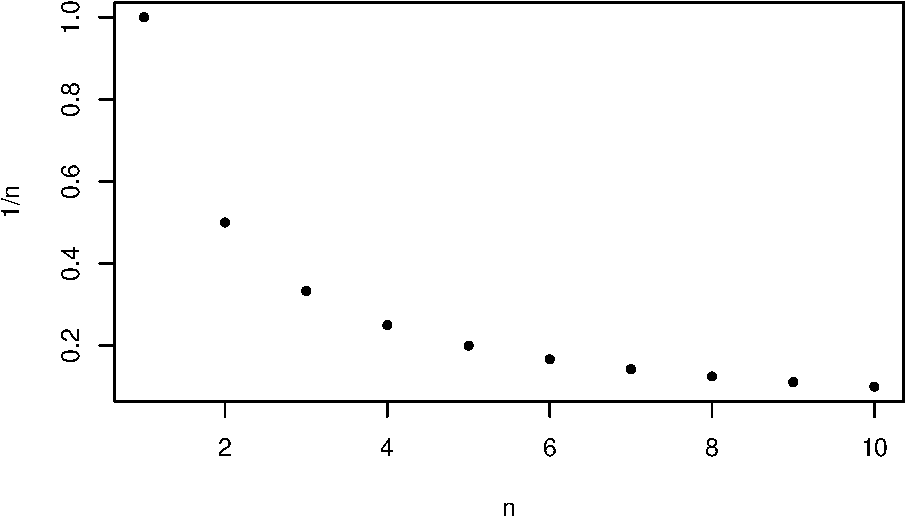
\includegraphics{_main_files/figure-latex/chunk-label-1.pdf}
\caption{\label{fig:chunk-label}Les premières valeurs de la suite de terme général \(x_n=1/n\) qui converge vers 0.}
\end{figure}

\begin{proposition}

Soit \((x_n)\) et \((y_n)\) deux suites convergentes de limites respectives \(\ell_1\) et \(\ell_2\). On a les propriétés suivantes.

\begin{enumerate}
\def\labelenumi{\arabic{enumi}.}
\tightlist
\item
  La suite \(x_n+y_n\) est convergente avec \(\lim x_n+y_n=\ell_1+\ell_2\).
\item
  La suite \(x_ny_n\) est convergente avec \(\lim x_ny_n=\ell_1\ell_2\).
\item
  Si \(\ell_2\neq0\) alors la suite \(x_n/y_n\) est convergente avec \(\lim x_n/y_n=\ell_1/\ell_2\).
\item
  Si \(x_n\leq y_n\) pour tout \(n\in\mathbb{N}\) alors \(\ell_1\leq \ell_2\).
\end{enumerate}

\end{proposition}

\hypertarget{opuxe9rations-sur-les-limites}{%
\section{Opérations sur les limites}\label{opuxe9rations-sur-les-limites}}

\begin{definition}[Bornes supérieures et inférieures]
Si \((x_n)\) est une suite majorée, on note \(\sup x_n\) le plus petit des ses majorants.

Si \((x_n)\) est une suite minorée, on note \(\inf x_n\) le plus petit des ses minorants.
\end{definition}

L'existence des ces bornes supérieures (\(\sup x_n\)) et inférieures (\(\inf x_n\)) n'est pas évidente et une conséquence d'une construction formelle de l'ensemble des nombres réels \(\mathbb{R}\). Nous ne rentrons pas dans ces détails et admettons l'existence des bornes supérieures et inférieures. La construction donne la proposition suivante.

\begin{proposition}
\protect\hypertarget{prp:sup}{}\label{prp:sup}Soit \((x_n)\) une suite majorée (respectivement minorée) de borne supérieure \(A=\sup x_n\) (respectivement borne inférieure \(A=\inf x_n\)) et \(\varepsilon>0\) . Alors il existe \(n\in\mathbb{N}\) tel que \(x_n\geq A-\varepsilon\) (respectivement \(x_n\leq A+\varepsilon\)).
\end{proposition}

\begin{proposition}
Toute suite \((x_n)\) croissante et majorée est convergente vers \(\sup x_n\).
\end{proposition}

\begin{proposition}
Toute suite \((x_n)\) décroissante et minorée est convergente vers \(\inf x_n\).
\end{proposition}

\begin{proof}
La preuve est la même pour les deux proposition en changeant ce qui doit l'être. On prouve seulement la première et on note \(A=\sup x_n\). Soit \(\varepsilon>0\), par la Proposition \ref{prp:sup}, il existe \(n_0\in\mathbb{N}\) tel que \(x_{n_0}\geq A-\varepsilon\).Par croissance, on a aussi \(x_n\geq x_{n_0}\geq A-\varepsilon\) pour \(n\geq n_0\). Comme \(A\) est un majorant, on a aussi \(x_{n}\leq A\) pour tout \(n\in\mathbb{N}\) et donc \(n\in\mathbb{N}\).
\end{proof}

\begin{example}
La suite \((x_n)\) définie par \(x_n=1/n\) pour \(n\in\mathbb{N}^*\) est décroissante et minorée par 0. On a déjà vu qu'elle converge vers 0 dans l'Exemple \ref{exm:harmonique}.
\end{example}

\hypertarget{limites-infinies}{%
\section{Limites infinies}\label{limites-infinies}}

Il existe des cas où une suite ne converge pas mais devient ``aussi grande possible''. La définition suivante rend rigoureuse cette notion.

\begin{definition}
Une suite \((x_n)\) \emph{converge vers \(+\infty\)} si pour tout \(A>0\), il existe \(N\in\mathbb{N}\) tel que pour tout \(n\geq N\), \(x_n\geq A\). On note \(\lim x_n=+\infty\).

Une suite \((x_n)\) \emph{converge vers \(-\infty\)} si pour tout \(A<0\), il existe \(N\in\mathbb{N}\) tel que pour tout \(n\geq N\), \(x_n\leq A\). On note \(\lim x_n=-\infty\).
\end{definition}

\begin{example}
Pour un entier srictement positif \(k\), la suite \((x_n)\) où \(x_n=n^k\) converge vers \(+\infty\).
\end{example}

\begin{proof}
Soit \(A>0\), On choisit \(N\geq A\) et \(N\geq1\), par exemple, \(N=\lfloor A\rfloor+1\) (partie entière plus 1). Pour \(n\geq N\), on a \(n^k=\underbrace{n\times\cdots\times n}_{k\ \textrm{fois}}\geq n\geq N\geq A\) car \(n\geq 1\) et \(k\geq 1\).
\end{proof}

\begin{proposition}
Une suite croissante non majorée converge vers \(+\infty\). De même, une suite décroissante non minorée converge vers \(-\infty\).
\end{proposition}

\begin{proof}
On prouve uniquement le cas d'une suite croissante, la preuve s'adapte pour le cas décroissant. Soit \((x_n)\) une suite croissante non majorée. Soit \(A>0\). Comme la suite n'est pas pas majorée, \(A\) n'est pas un majorant et donc il existe \(n_0\in\mathbb{N}\) tel que \(x_{n_0}>A\) et donc par croissance, pour tout \(n\geq n_0\), \(x_n\geq A\). Ce qui montre bien \(\lim x_n=+\infty\).
\end{proof}

\hypertarget{deux-exemples}{%
\section{Deux exemples}\label{deux-exemples}}

\hypertarget{suites-arithmuxe9tiques}{%
\subsection{Suites arithmétiques}\label{suites-arithmuxe9tiques}}

\begin{theorem}

Soit \((x_n)\) une suite arithmétique de raison \(r\)

\begin{itemize}
\tightlist
\item
  Si \(r>0\) alors \(\lim x_n=+\infty\).
\item
  Si \(r=0\) alors \(\lim x_n=x_0\).
\item
  Si \(r<0\) alors \(\lim x_n=-\infty\).
\end{itemize}

\end{theorem}

\begin{proof}
Par récurrence, on montre que \(x_n=x_0+nr\).

\begin{itemize}
\tightlist
\item
  Si \(r>0\) alors pour \(A>0\) fixé, on prend \(N=\lfloor (A-x_0)/r\rfloor+1\) et alors pour \(n\geq N\), \(n\geq (A-x_0)/r\), ce qui donne \(x_n=x_0+nr\geq A\) et donc \(\lim x_n=+\infty\).
\item
  Si \(r=0\) alors la suite \((x_n)\) est constante égale à \(x_0\) et converge donc vers cette limite.
\item
  Si \(r<0\) alors pour \(A<0\) fixé, on prend \(N\) entier plus grand que \((A-x_0)/r\) (remarquons que \(A/r>0\) car \(A\) et \(r\) sont négatifs). Maintenant, pour \(n\geq N\), \[n\geq \frac{A-x_0}{r}\] et comme \(r<0\),
\end{itemize}

\[nr\leq A-x_0\]
et donc \(x_n=x_0+nr\leq A\). Ainsi, \(\lim x_n=-\infty\).
\end{proof}

\hypertarget{suites-guxe9omuxe9triques}{%
\subsection{Suites géométriques}\label{suites-guxe9omuxe9triques}}

Dans le théorème suivant, on se place dans le cas d'une suite géométrique de premier terme \(x_0\) non nul. En effet, si \(x_0=0\), la suite est constante égale à 0 et il n'y a rien de plus à dire.

\begin{theorem}

Soit \((x_n)\) une suite géométrique de raison \(r\) avec \(x_0\neq0\).

\begin{itemize}
\tightlist
\item
  Si \(r>1\) alors \(\lim x_n=+\infty\) si \(x_0>0\) et \(\lim x_n=-\infty\) si \(x_0<0\).
\item
  Si \(r=1\) alors la suite est constante égale à \(x_0\).
\item
  Si \(|r|<1\) alors \(\lim x_n=0\).
\item
  Si \(r\leq -1\) alors la suite \((x_n)\) n'est pas convergente.
\end{itemize}

\end{theorem}

\begin{proof}

Un raisonnement par récurrence montre que \(x_n= r^nx_0\).

\begin{itemize}
\tightlist
\item
  Si \(r>1\) alors posons \(a=r-1>0\). Ainsi, \(r^n=(1+a)^n\geq 1+na\). Pour \(A>0\), On choisit \(N\) entier supérieur à \(A/a\), ainsi pour \(n\geq N\), \(n\geq A/a\) et donc \$r\^{}n\geq
\item
  Si \(r=1\) alors \(r^n=1\) pour tout \(n\) et donc \(x_n=x_0\) pour tout \(n\).
\item
\item
  Si \(r\leq -1\) alors \(r^{2n}\) est positif mais \(r^{2n+1}\) est négatif
\end{itemize}

\end{proof}

\hypertarget{suites-adjacentes}{%
\section{Suites adjacentes}\label{suites-adjacentes}}

\begin{definition}
Soit \((x_n)\) et \((y_n)\) deux suites numériques. On dit que ces suites sont \emph{adjacentes} si \(x_n\geq y_n\) pour tout \(n\in\mathbb{N}\), \((x_n)\) est croissante, \((y_n)\) est décroissante et \(\lim y_n-x_n=0\).
\end{definition}

\begin{proposition}
Si \((x_n)\) et \((y_n)\) sont deux suites adjacentes alors ces deux suites sont convergentes et \(\lim x_n=\lim y_n\).
\end{proposition}

\begin{proof}
La suite \((x_n)\) est croissante majorée (par \(y_0\) par exemple) et donc converge vers une limite \(\ell_1\). De même, \((y_n)\) est décroissante minorée et donc converge vers une limite \(\ell_2\). Ainsi la suite \((y_n-x_n)\) est convergente de limite \(\ell_2-\ell_1\). Comme \(\lim y_n-x_n=0\), on a \(\ell_2-\ell_1=0\) et donc \(\ell_1=\ell_2\).
\end{proof}

\begin{figure}
\centering
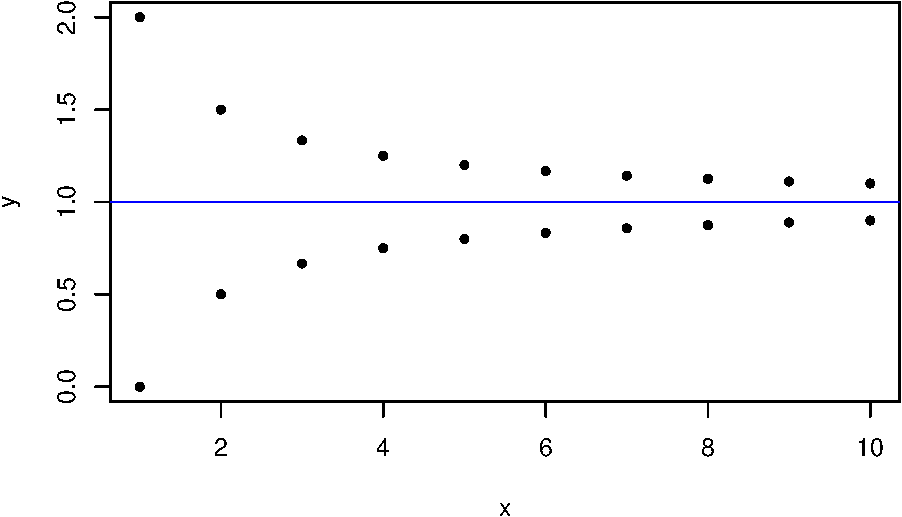
\includegraphics{_main_files/figure-latex/chunk-label-1-1.pdf}
\caption{\label{fig:chunk-label-1}Deux suites adjacentes qui converge vers 1.}
\end{figure}

\begin{theorem}[Théorème des gendarmes]
Soit \((x_n), (y_n)\) et \((u_n)\) trois suites telles que pour tout \(n\in\mathbb{N}\), \(x_n\leq u_n\leq y_n\) et telles \((x_n), (y_n)\) sont convergentes avec \(\lim x_n=\lim y_n=\ell\) alors \((u_n)\) est convergente de limite \(\ell\).
\end{theorem}

\hypertarget{exercices}{%
\section{Exercices}\label{exercices}}

\begin{exercise}
Donner un exemple d'une suite qui n'est pas monotone.
\end{exercise}

\begin{exercise}
Montrer qu'une suite \((x_n)\) est bornée si et seulement s'il existe \(A\geq 0\) tel que pour tout \(n\in \mathbb{N}\), \(|x_n|\leq A\)
\end{exercise}

\begin{exercise}
On définit deux suites \((x_n)\) et \((y_n)\) par \(x_n=2^n\) et \(y_n=3^n\). Déterminer la comportement des suites de termes généraux \(z_n=x_n+y_n\), \(u_n=x_n-y_n\), \(v_n=x_ny_n\), \(w_n=x_n/y_n\) et \(t_n=y_n/x_n\).
\end{exercise}

\begin{exercise}
Soit \((x_n)\) une suite convergente de limite \(\ell\). On pose \(y_n=x_{2n}\) pour tout \(n\in\mathbb{N}\). Montrer que la suite \((y_n)\) est convergente de limite \(\ell\).
\end{exercise}

\begin{exercise}

Soit \(a,b\in \mathbb{R}\). On fixe \(x_0\) et on définit récursivement \(x_{n+1}=ax_n+b\).

\begin{enumerate}
\def\labelenumi{\arabic{enumi}.}
\tightlist
\item
  Déterminer le comportement de \((x_n)\) si \(a=0\) ou \(a=1\).
\item
  On suppose \(a\neq0\). On pose \(c=\frac{b}{a-1}\) et \(y_n=x_n+c\). Montrer que \((y_n)\) est une suite géométrique de raison \(a\).
\item
  En fonction de \(a\), déterminer le comportement de \(y_n\) puis celui de \(x_n\).
\item
  À l'aide de la formule explicite d'une suite géométrique, déduire une formule explicite pour \(x_n\).
\end{enumerate}

\end{exercise}

\hypertarget{continuituxe9-et-duxe9rivation-de-fonctions-ruxe9elles}{%
\chapter{Continuité et dérivation de fonctions réelles}\label{continuituxe9-et-duxe9rivation-de-fonctions-ruxe9elles}}

\hypertarget{continuituxe9}{%
\section{Continuité}\label{continuituxe9}}

\hypertarget{duxe9rivation}{%
\section{Dérivation}\label{duxe9rivation}}

\hypertarget{suites-ruxe9currentes}{%
\chapter{Suites récurrentes}\label{suites-ruxe9currentes}}

\hypertarget{approximations}{%
\chapter{Approximations}\label{approximations}}

\hypertarget{notations-de-landau-et-type-de-complexituxe9}{%
\chapter{Notations de Landau et type de complexité}\label{notations-de-landau-et-type-de-complexituxe9}}

  \bibliography{book.bib,packages.bib}

\end{document}
